\documentclass{article}
\title{P5 Report}
\author{Nick Werle}
\usepackage{hyperref}
\usepackage{graphicx}

\begin{document}
\maketitle
\section{Preamble}
Files will be submitted per instructions to pilot, and all work will be available on github at: \url{https://github.com/NickWer/CEG3900_P5} in two days.

\section{Task 1}
Deliverables: See devDocs.pdf and userDocs.pdf, see images 1-4 for screenshots.

Status report: I believe my user docs are sufficient for this game. I believe my dev docs, while they are not super in depth, provide an adequate high level view of the application's classes. They do not address specific implementation details however.

Experience: The user docs were not bad. The game is kind of fun but the difficulty is low and then becomes somewhat impractically difficult after a certain point. Very hard to play while the phone is plugged in. The dev docs were kind of a pain, but realistically it's not too terrible to understand all the source code.

	\begin{figure}[ht]
		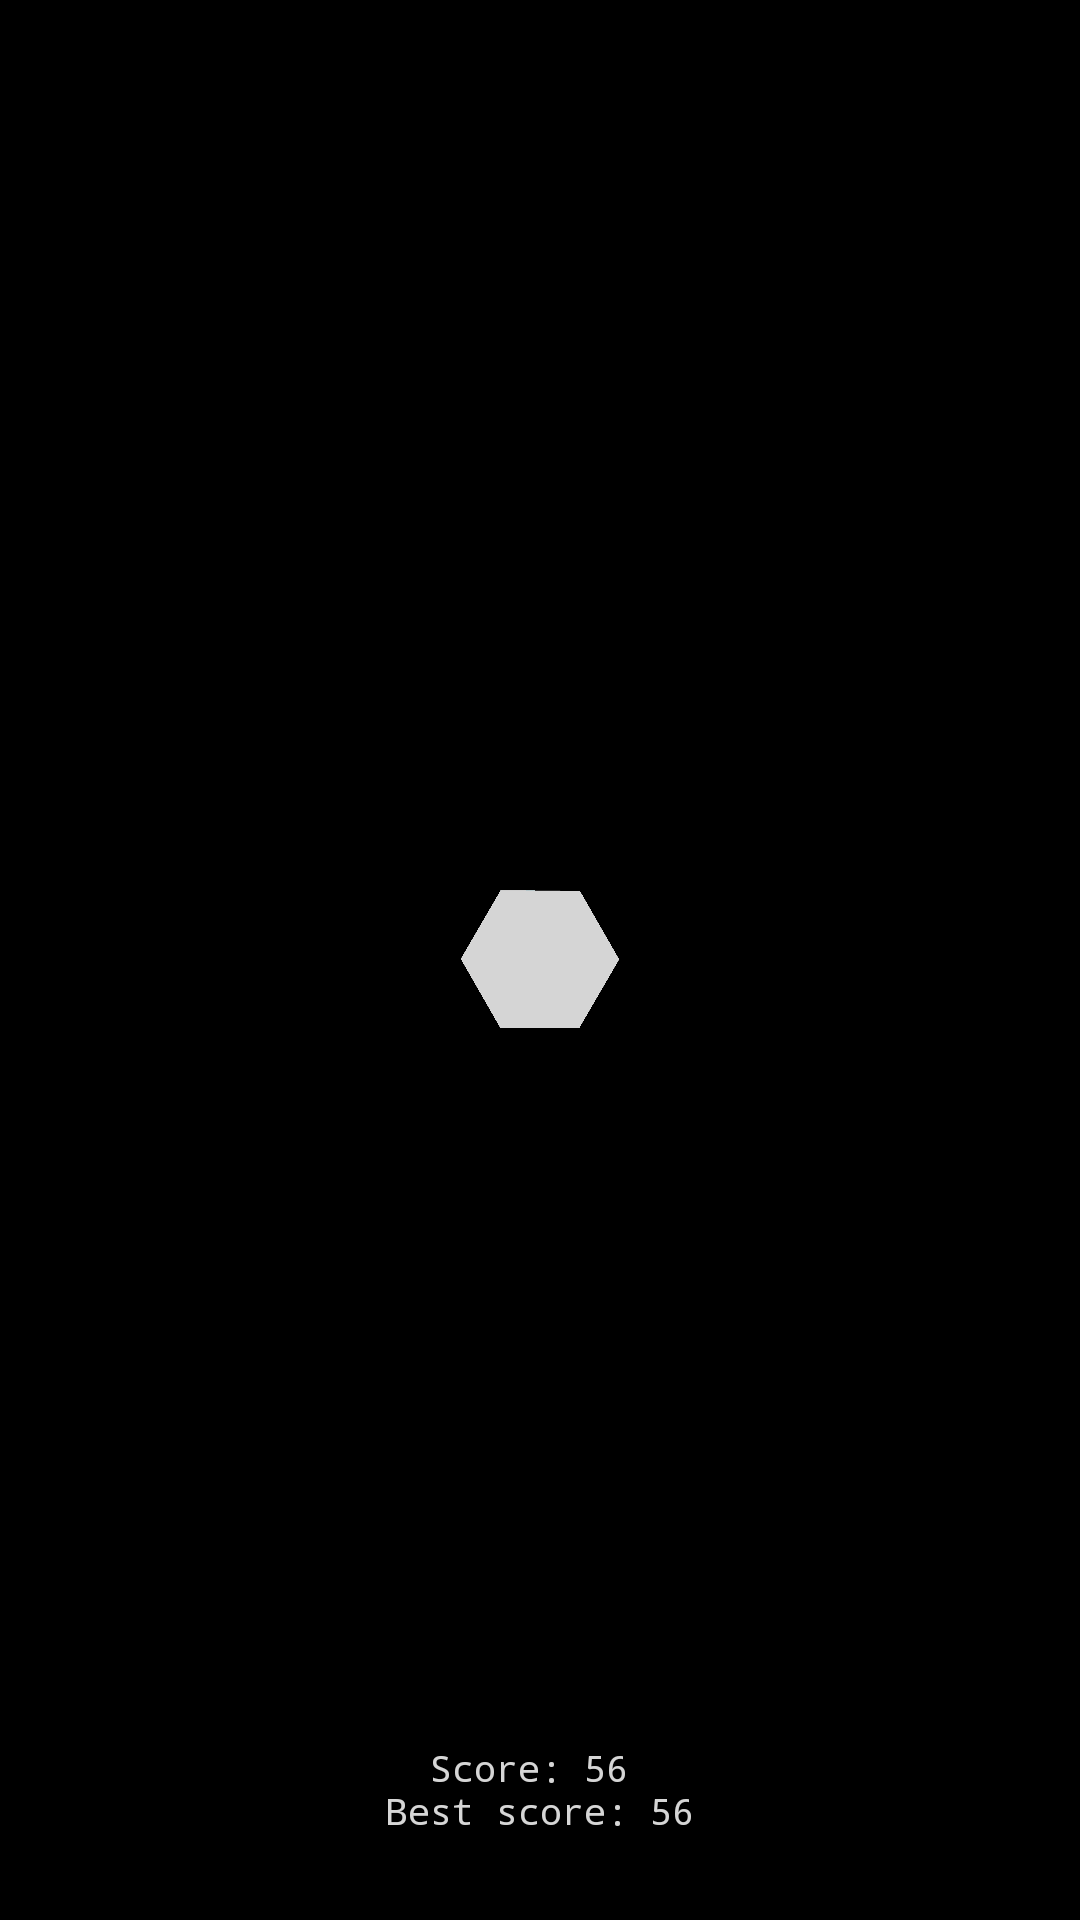
\includegraphics[width=3in]{img/t1s1.png}
		\centering
		\caption{Task 1 - Starting screen}
	\end{figure}
	\begin{figure}[ht]
		
\includegraphics[width=3in]{img/t1s2.png}
		\centering
		\caption{Task 1 - A game has begun - the center hexagon is much smaller}
	\end{figure}
	\begin{figure}[ht]
		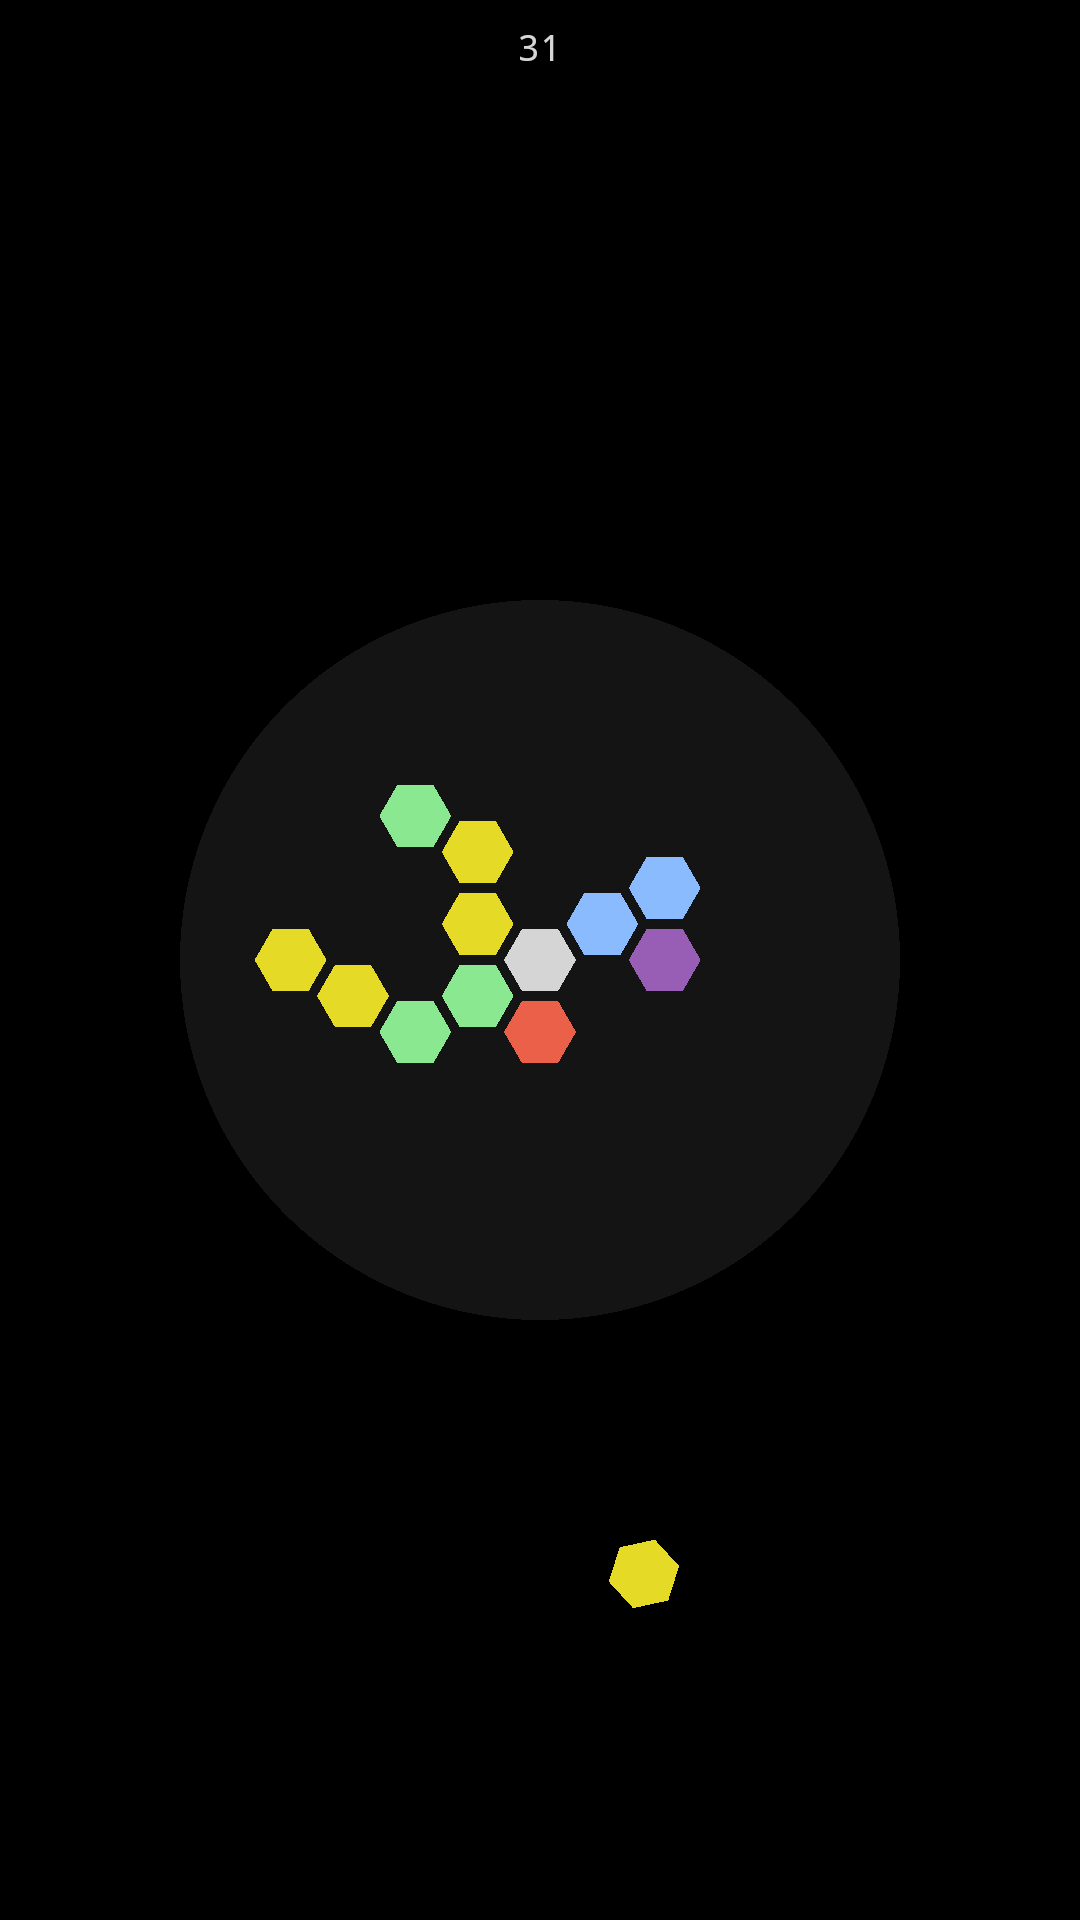
\includegraphics[width=3in]{img/t1s3.png}
		\centering
		\caption{Task 1 - Part 1 of 2 - Demonstrating how a chain can remove more than just 3 blocks}
	\end{figure}
	\begin{figure}[ht]
		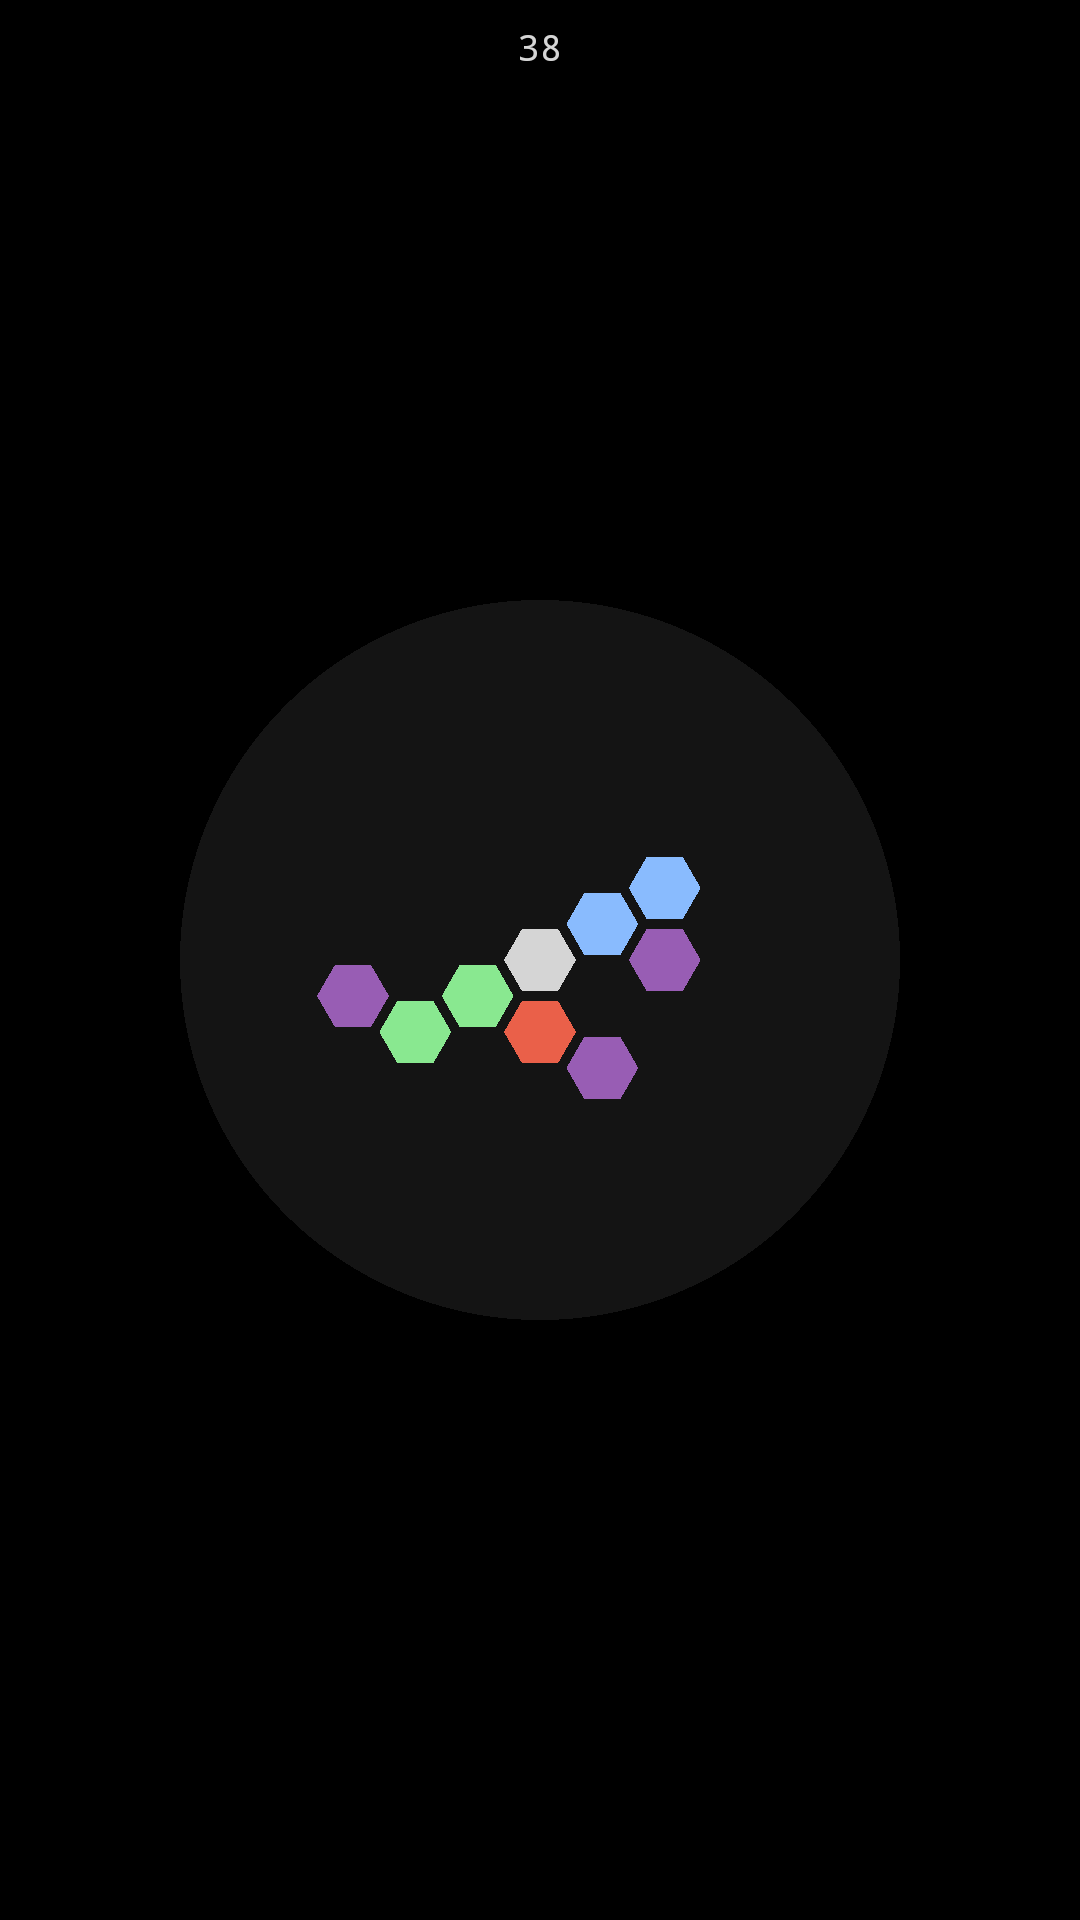
\includegraphics[width=3in]{img/t1s4.png}
		\centering
		\caption{Task 1 - Part 2 of 2 - Demonstrating how a chain can remove more than just 3 blocks}
	\end{figure}

\section{Task 2}
Deliverables: See screenshots 5-8. My MS Azure account is linked to my wright state email address, werle.3@wright.edu

Status Report: The application works as expected. Uploads and recalls images without hiccup.

Experience Report: Building the APK was very easy. Honestly registering to MS Azure was harder, because of a glitch with wright state's single sign on. I had to go incognito to get it to work. Other than that, and trying to find my account key, it was not a terrible experience. A promising platform, for sure, with a generous trial offer.

	\begin{figure}[ht]
		
\includegraphics[width=3in]{img/t2s1.png}
		\centering
		\caption{Task 2 - Starting screen}
	\end{figure}
	\begin{figure}[ht]
		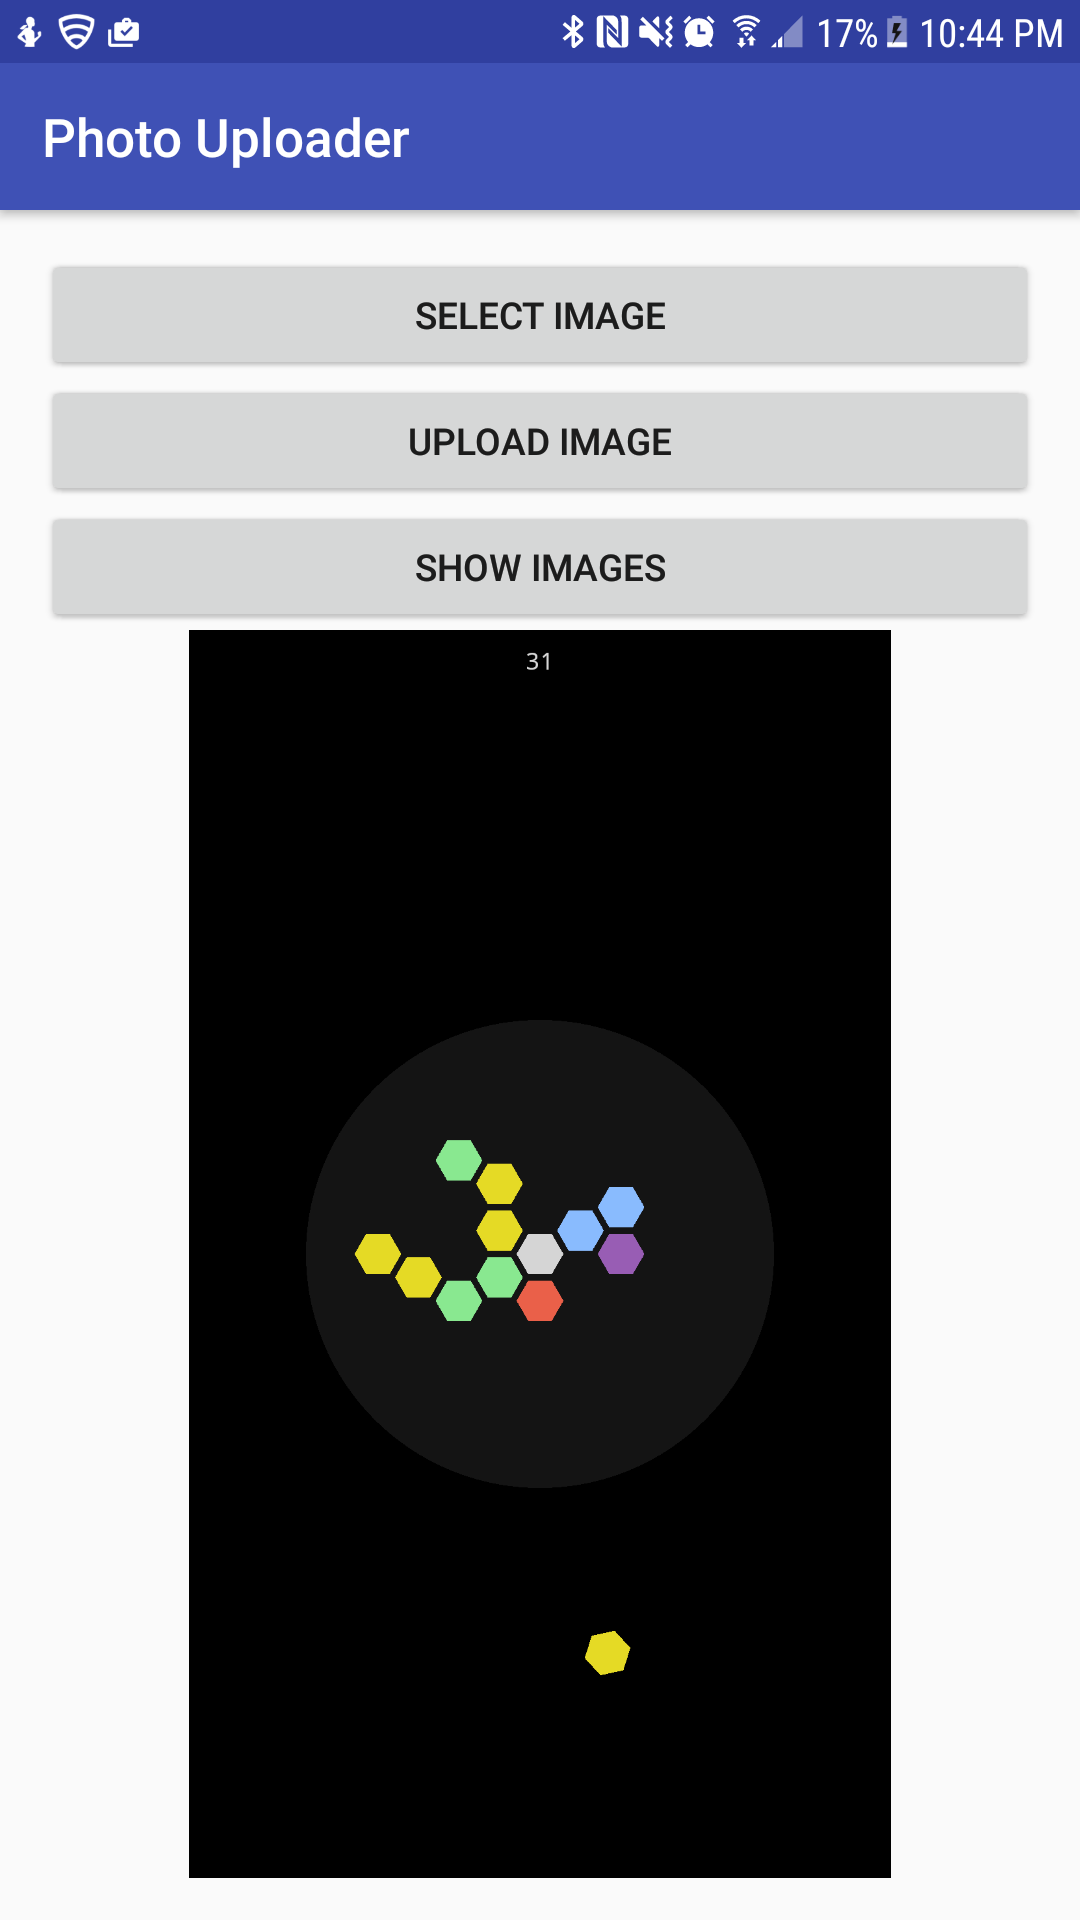
\includegraphics[width=3in]{img/t2s2.png}
		\centering
        \caption{Task 2 - An image about to be uploaded}
	\end{figure}
	\begin{figure}[ht]
		
\includegraphics[width=3in]{img/t2s3.png}
		\centering
        \caption{Task 2 - List of images that have been uploaded}
	\end{figure}
	\begin{figure}[ht]
		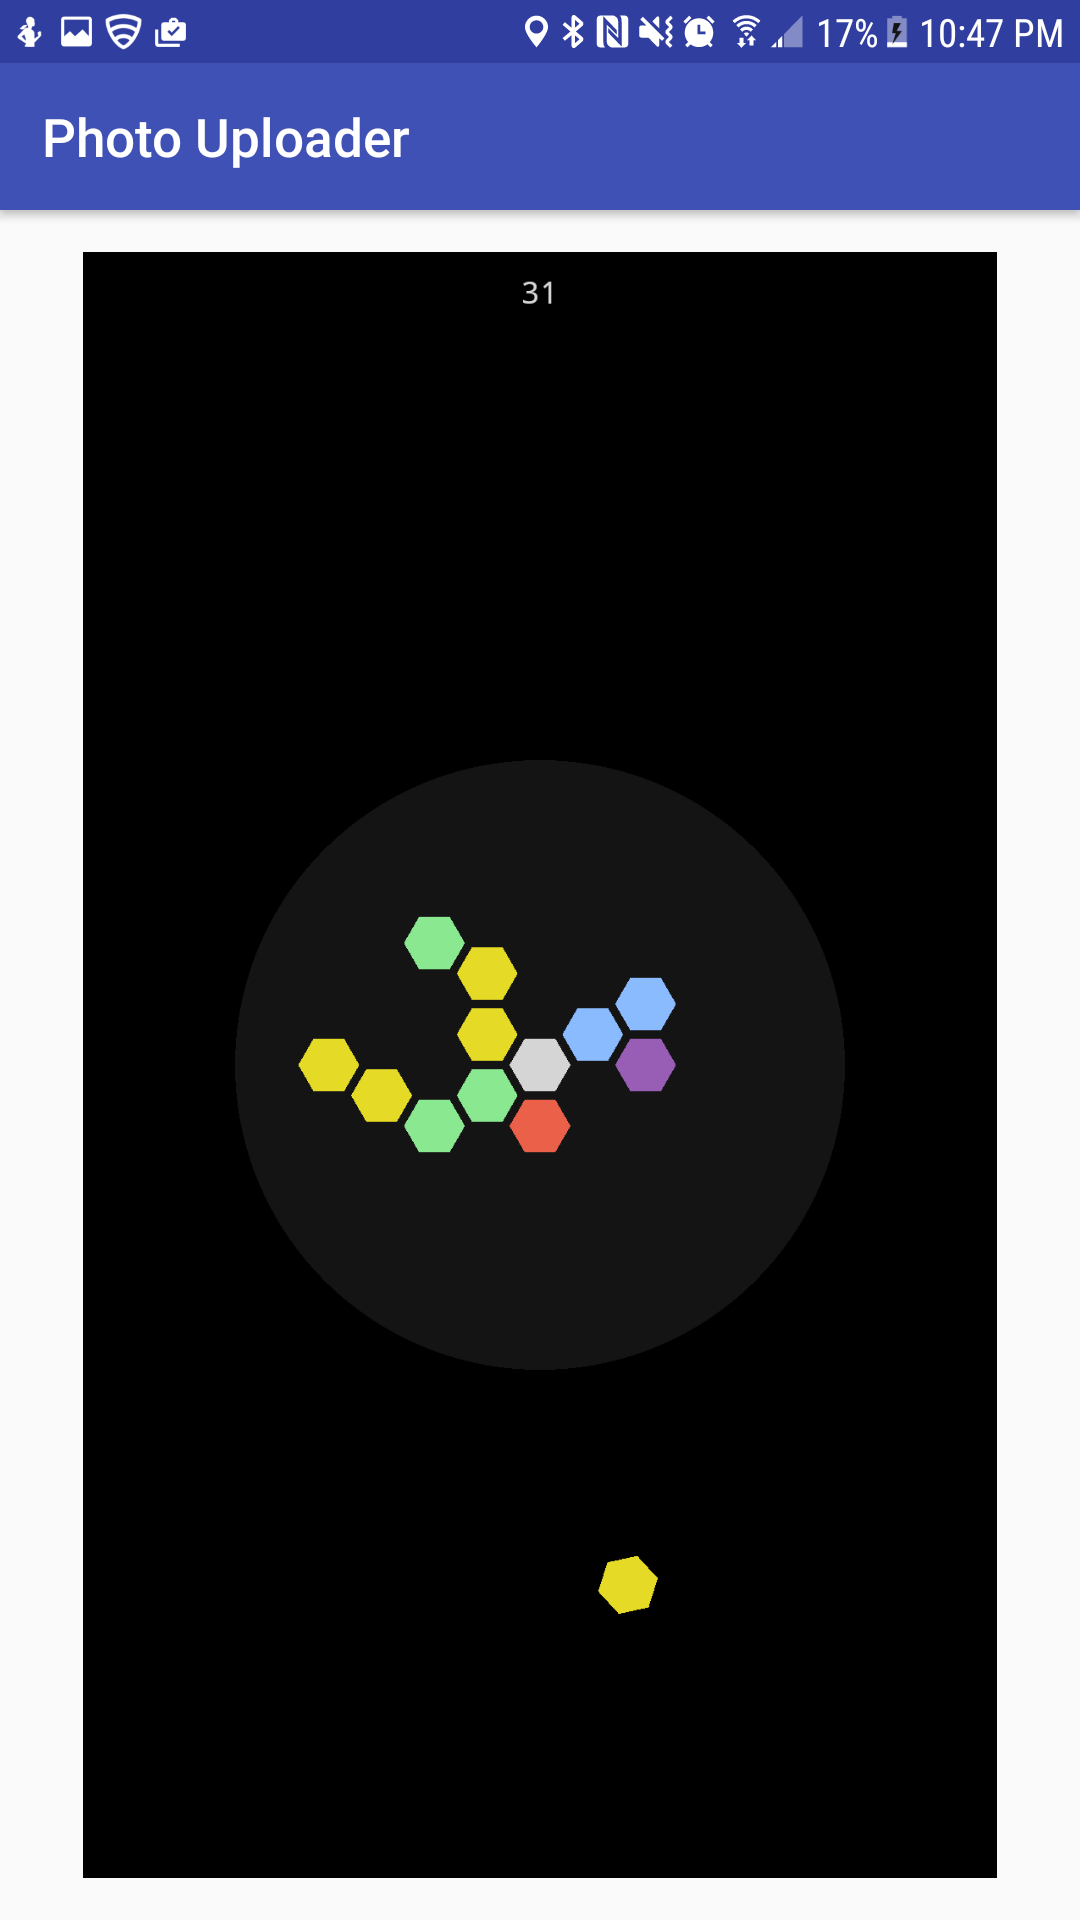
\includegraphics[width=3in]{img/t2s4.png}
		\centering
		\caption{Task 2 - The uploaded image}
	\end{figure}
\end{document}
